\documentclass{book}
\usepackage{commeunjeustyle}

\begin{document}
\chapter*{Déterminant}
\begin{Texte}%label=introduction_chapter
D'un point de vue géométrique, le déterminant de $n$ vecteurs $(\vec{v_1},\ldots,\vec{v_n})$ de $\R^n$ est le volume du parallélépipède engendré par ces $n$ vecteurs. Le déterminant d'une matrice  est le volume par ses vecteurs colonnes. Le déterminant d'un endomorphisme est le volume par l'image d'une base.\\
Il fut initialement introduit en algèbre, pour résoudre un système d'équations linéaires comportant autant d'équations que d'inconnues. Il se révèle être un outil très puissant dans de nombreux domaines. Il intervient ainsi dans l'étude des endomorphismes, la recherche de leurs valeurs propres, les propriétés d'indépendance linéaire de certaines familles de vecteurs, mais aussi dans le calcul différentiel, par exemple dans la formule de changement de variables dans les intégrales multiples.
\end{Texte}

\begin{Texte}%label=notation_chapter
Dans ce chapitre, un corps $\K$ désigne soit l'ensemble des nombres réels $\R$ ou soit l'ensemble des nombres complexes $\C$.
$\mathcal{B}_n$ désigne la base canonique de $\K^n$.  
\end{Texte}
\begin{Exemple}[Tailles d'un père et d'un fils] %label=introduction
La somme des tailles d'un fils et du père est de 2,5 mètres. La différence de tailles  est de 0.5 mètres.
Quel est la taille du fils et du père ? \\
Soit la variable $x$ représentant la taille du fils et la variable $y$ représentant la taille du père.\\
Le couple $(x,y)$ vérifie le système suivant  :
$$(S)\quad \begin{cases}
x+y&=2,5\\
-x+y&=0,5
\end{cases}
$$
Avant de déterminer explicitement la solution, un mathématicien se pose des questions sur la structure des solutions du problème. Comme vu au chapitre sur les espaces vectoriels, le système $(S)$ est équivalent à :
$$	
%\begin{pmatrix}
% 1  & 1  \\ 
% -1 &1   \\
%\end{pmatrix}\times\begin{pmatrix}
%  {\color{red}x}   \\
%  {\color{green}y} \\
%\end{pmatrix}=\begin{pmatrix}
% {\color{blue}2,5}   \\
% {\color{blue}0,5}  \\
%\end{pmatrix}
%\Leftrightarrow
	 {\color{red}x}\begin{pmatrix}
 1    \\
 -1   \\
\end{pmatrix}+{\color{green}y}\begin{pmatrix}
  1   \\
  1  \\
\end{pmatrix}=\begin{pmatrix}
 {\color{blue}2,5}   \\
 {\color{blue}0,5}  \\
\end{pmatrix}$$
En d'autres terme, on cherche les combinaisons linéaires des $(\begin{pmatrix}
 1    \\
 -1   \\
\end{pmatrix},\begin{pmatrix}
 1   \\
  1  \\
\end{pmatrix})$ égales au vecteur $\begin{pmatrix}
 {\color{blue}2,5}   \\
 {\color{blue}0,5}  \\
\end{pmatrix}$
\begin{center}
\begin{tikzpicture}[general,scale=1.5]
\draw [quadrillage] (-0.1,-1.1) grid (3,1.1);
\node[below left,,color=black!70] (0,0) {$O$};
\draw[->,color=black!70] (0,0) -- (1,0) node[below] {$\vec{e_1}$};
\draw[->,color=black!70] (0,0) -- (0,1) node[left] {$\vec{e_2}$};
\draw [->, epais] (0,0) -- (1,-1)node[right]{$\begin{pmatrix}
 1    \\
 -1   \\
\end{pmatrix}$};
\draw [->, epais] (0,0) -- (1,1)node[right]{$\begin{pmatrix}
 1    \\
 1   \\
\end{pmatrix}$};
\draw [->, epais] (0,0) -- (2.5,0.5)node[right]{$\begin{pmatrix}
 {\color{blue}2,5}   \\
 {\color{blue}0,5}  \\
\end{pmatrix}$};
\draw [->, epais] (0,0) -- (2.3,-0.5)node[right]{$ {\color{red}x}\begin{pmatrix}
 1    \\
 -1   \\
\end{pmatrix}+{\color{green}y}\begin{pmatrix}
  1   \\
  1  \\
\end{pmatrix}$};
\end{tikzpicture}
\end{center}
De deux choses l'une :
\begin{itemize}
\item si la famille est une base, alors il existe une unique solution,
\item si la famille n'est pas une base, alors soit il n'existe pas de solution ou une infinité.   
\end{itemize}
En dimension 2,  si les deux vecteurs  ne sont pas colinéaires alors ils forment une base et on a donc existence et unicité de la solution.  Dans notre exemple,  comme les deux vecteurs  $\begin{pmatrix}
 1    \\
 -1   \\
\end{pmatrix}$ et $\begin{pmatrix}
 1   \\
  1  \\
\end{pmatrix}$ ne sont pas colinéaires, il y a existence et  unicité de la  solution.\\
L'idée du déterminant est d'avoir un outil permettant de répondre à cette question : est-ce qu'une famille de $n$ vecteurs est une base  en dimension $n$ ?\\
Dans le plan, le déterminant calcule l'aire orientée du parallélogramme défini par deux vecteurs, $\Vect{u}=\begin{pmatrix}
a\\c
\end{pmatrix}$ et $\Vect{v}=\begin{pmatrix}
b\\d
\end{pmatrix}$  
\begin{center}
\begin{tikzpicture}[scale=1.3,>=latex]
\filldraw[colorprop!20,draw=colorprop,dashed] (0,0) -- (2.2,0.3) -- (2.6,1.5) -- (0.4,1.2) -- cycle;
\draw[->,colorprop,thick] (0,0) -- (2.2,0.3) node[right] {$\vec{u}$};
\draw[->,colorprop,thick] (0,0) -- (0.4,1.2) node[above] {$\vec{v}$};
\node[below left,color=black!70] (0,0) {$O$};
\draw[->,color=black!70] (0,0) -- (0.5,0) node[below] {$\vec{e_1}$};
\draw[->,color=black!70] (0,0) -- (0,0.5) node[left] {$\vec{e_2}$};
\end{tikzpicture}
\end{center}
Si les deux vecteurs sont colinéaires, alors l'aire est égale à 0 car la parallélogramme est aplati  sinon l'aire est différente de zéro. C'est-à-dire, la famille $(\Vect{u},\Vect{v})$ est une base si et seulement si le déterminent est différent de zéro. \\
Dans l'espace,  le déterminant calcule le volume du parallélépipède : 
\begin{center}
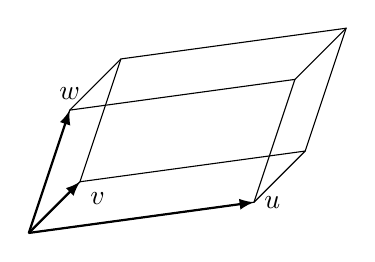
\begin{tikzpicture}[scale=1.3,>=latex]
\draw (0,0) -- (2.2,0.3) -- (2.6,1.5) -- (0.4,1.2) -- cycle;
\draw (0.5,0.5) -- (2.7,0.8) -- (3.1,2.0) -- (0.9,1.7) -- cycle;
\draw (0,0) -- (0.5,0.5);
\draw (2.2,0.3) -- (2.7,0.8);
\draw (2.6,1.5) --  (3.1,2.0);
\draw  (0.4,1.2) --  (0.9,1.7);

\draw[->,thick] (0,0) -- (2.2,0.3) node[right] {$\Vect{u}$};
\draw[->, thick ] (0,0) -- (0.5,0.5) node[below right] {$\Vect{v}$};
\draw[->,thick] (0,0) -- (0.4,1.2) node[above] {$\Vect{w}$};
\end{tikzpicture}
\end{center} 
De nouveau, la famille $(\Vect{u},\Vect{v},\Vect{w})$ est une base si et seulement si le déterminent est différent de zéro.\\
Pour pouvoir appliquer cet outil, il nous faut une formule exprimant le volume en fonction des coordonnées des vecteurs.
\begin{Proposition}[Aire du parallélogramme]
L'aire orientée du parallélogramme est donnée par :  
$$
\Fonction{\det_{\mathcal{B}_2}}{\R^2\times\R^2}{\R}{\begin{pmatrix}
a\\c
\end{pmatrix},\begin{pmatrix}
b\\d
\end{pmatrix}}{\begin{vmatrix}
a & b \\
c & d
\end{vmatrix}=a d-c d}.
$$
\end{Proposition}
\begin{Demonstration}
\begin{itemize} 
\item $\vec{u}$ et $\vec{v}$ colinéaires :
le parallélogramme est aplati, donc le déterminant (l'aire) nulle.
\item $\vec{u}$ et $\vec{v}$ non colinéaires :
\begin{itemize} 
\item $\vec{u}$ et $\vec{v}$ colinéaires aux vecteurs de la base : supposons que 
$\vec{u}=\left(\begin{smallmatrix}a\\0\end{smallmatrix}\right)$ et
$\vec{v}\left(\begin{smallmatrix}0\\d\end{smallmatrix}\right)$. Alors le parallélogramme est un rectangle de côtés $a$ et $d$, donc le déterminant (l'aire)
$ad$.

\begin{center}
\begin{tikzpicture}[scale=1.3,>=latex]

\filldraw[colorprop!20,draw=colorprop,dashed] (0,0) -- (2.2,0) -- (2.2,1.2) -- (0,1.2) -- cycle;
\draw[->,colorprop,thick] (0,0) -- (2.2,0) node[right ] {$\vec{u}$};
\draw[->,colorprop,thick] (0,0) -- (0,1.2) node[above] {$\vec{v}$};

\node[below] at (2.2,0) {$a$};
\node[left] at (0,1.2) {$d$};

\node[below left,color=black!50] (0,0) {$O$};
\draw[->,color=black!50] (0,0) -- (0.5,0) node[below] {$\vec{e_1}$};
\draw[->,color=black!50] (0,0) -- (0,0.5) node[left] {$\vec{e_2}$};

\end{tikzpicture}
\end{center}
\item cas générale :
Notons $\vec{u}= \left(\begin{smallmatrix}a\\c\end{smallmatrix}\right)$ et
$\vec{v} =\left(\begin{smallmatrix}b\\d\end{smallmatrix}\right)$.
Si $a\neq0$, alors $\vec{v'}=\vec{v}-\frac{b}{a}\vec{u}$ est un vecteur vertical:
$\vec{v'}=\left(\begin{smallmatrix}0\\d-\frac{b}{a}c\end{smallmatrix}\right)$.
L'opération  de remplacer $\vec{v}$ par $\vec{v'}$ ne change
pas l'aire du parallélogramme (remplacer le triangle vert
par le triangle rouge).
\begin{center}
\begin{tikzpicture}[scale=1.3,>=latex]

\filldraw[colordef!40,draw=colordef,dashed] (0,0) -- (0,1.145) -- (0.4,1.2)  -- cycle;

\filldraw[colorprop!20,draw=colorprop,dashed] (0,0) -- (2.2,0.3) -- (2.6,1.5) -- (0.4,1.2) -- cycle;
\fill[green!40] (2.2,0.3) -- (2.6,1.5) -- (2.2,1.445)  -- cycle;
\draw[green] (2.2,0.3) -- (2.2,1.445);
\draw[green] (2.2,0.3) -- (2.6,1.5) -- (2.2,1.445) ;
\draw[->,colorprop,thick] (0,0) -- (2.2,0.3) node[right] {$\vec{u}$};
\draw[->,colorprop,thick] (0,0) -- (0.4,1.2) node[above] {$\vec{v}$};
\draw[->,thick] (0,0) -- (0,1.145) node[left] {$\vec{v'}$};

\node[below left,color=black!50] (0,0) {$O$};
\draw[->,color=black!50] (0,0) -- (0.5,0) node[below] {$\vec{e_1}$};
\draw[->,color=black!50] (0,0) -- (0,0.5) node[left] {$\vec{e_2}$};
\end{tikzpicture}
\end{center}
Ainsi, 
$$\det_{\mathcal{B}_2} (\vec{u},\vec{v})=\det (\vec{u},\vec{v'}).$$
On pose alors
$\vec{u'}= \left(\begin{smallmatrix}a\\0\end{smallmatrix}\right)$: c'est un vecteur horizontal.
Encore une fois l'opération de remplacer $\vec{u}$ par $\vec{u'}$ ne change par l'aire du parallélogramme

\begin{center}
\begin{tikzpicture}[scale=1.3,>=latex]
\filldraw[colorprop!20,draw=colorprop,dashed] (0,0) -- (0,1.145) -- (2.2,1.445)  -- (2.2,0.3) -- cycle;
\draw[->,colorprop,thick] (0,0) -- (2.2,0.3) node[right] {$\vec{u}$};
\draw[->,colorprop,thick] (0,0) -- (0,1.145) node[left] {$\vec{v'}$};
\draw[->,colordef,thick] (0,0) -- (2.2,0) node[below] {$\vec{u'}$};
\filldraw[colordef!70,draw=colordef,fill opacity=0.5,dashed] (0,0) -- (2.2,0) -- (2.2,1.145) -- (0,1.145) -- cycle;
\node[below left,color=black!50] (0,0) {$O$};
\draw[->,color=black!50] (0,0) -- (0.5,0) node[below] {$\vec{e_1}$};
\draw[->,color=black!50] (0,0) -- (0,0.5) node[left] {$\vec{e_2}$};
\end{tikzpicture}
\end{center}
Ainsi, 
$$\det_{\mathcal{B}_2} (\vec{u},\vec{v'})=\det_{\mathcal{B}_2} (\vec{u'},\vec{v'})\overbrace{=}^{\text{Aire du rectangle}}a(d-\frac{b}{a}c)=ad-bc.$$
\end{itemize}
\end{itemize}
\end{Demonstration}
Avec des arguments géométriques, on pourrait démontrer  que le volume  orientée du parallélépipède est donnée par :  
$$
\Fonction{\det_{\mathcal{B}_2}}{\R^3\times\R^3\times\R^3}{\R}{\begin{pmatrix}
a\\b\\g
\end{pmatrix},\begin{pmatrix}
b\\e\\h
\end{pmatrix},\begin{pmatrix}
c\\f\\i
\end{pmatrix}}{\begin{vmatrix}
a & b &c \\
d & e &f \\
g & h &i\\
\end{vmatrix}=a(ei-hf)-d(bi-hc)+g(bf-ec) }.
$$
En revanche en  dimension $n$ quelconque, il semble extrêmement difficile de déterminer la formule du volume à base d'arguments géométriques. Une brillante idée est  de déterminer un système d'équations fonctionnelles vérifié par le déterminant et d'en déduire la formule du volume. \\
En effet,  sur le plan, on remarque que l'aire est :
\begin{enumerate}
\item \impo{Normalisée} : l'aire du carré unité est 1, $\det({\mathcal{B}_2})=1$
\item \impo{2-linéaire} : linéaire par rapport à chaque une de ses deux variables.\\
Pour la linéarité à gauche, on a :
\begin{center}
\begin{tikzpicture}[scale=1.3,>=latex]
\filldraw[colorprop!20,draw=colorprop,dashed] (0,0) -- (2.2,0.3) -- (2.6,1.5) -- (0.4,1.2) -- cycle;
\filldraw[colordef!20,draw=colordef, opacity=0.2,dashed] (0,0) -- (1.1,0.15) -- (1.5,1.35) -- (0.4,1.2) -- cycle;
\draw[->,colorprop,thick] (0,0) -- (2.2,0.3) node[below] {$\lambda\vec{u}$};
\draw[->,colordef,thick] (0,0) -- (1.1,0.15) node[below] {$\vec{u}$};

\draw[->,colorprop,thick] (0,0) -- (0.4,1.2) node[above] {$\vec{v}$};

\node[below left,color=black!70] (0,0) {$O$};
\draw[->,color=black!70] (0,0) -- (0.5,0) node[below] {$\vec{e_1}$};
\draw[->,color=black!70] (0,0) -- (0,0.5) node[left] {$\vec{e_2}$};
\end{tikzpicture}\\
${\color{colorprop}\det_{\mathcal{B}_2}(\lambda\Vect{u},\Vect{v})}=\lambda{\color{colordef}\det_{\mathcal{B}_2}(\Vect{u},\Vect{v})}$\\
\begin{tikzpicture}[scale=1.3,>=latex]
\filldraw[colorprop!50,draw=colorprop, opacity=0.2,dashed] (0,0) -- (1.1,0.15) -- (1.5,1.35) -- (0.4,1.2) -- cycle;
\filldraw[colordef!50,draw=colordef, opacity=0.2,dashed] (1.1,0.15) -- (2.4,0.7) -- (2.8,1.9) -- (1.5,1.35) -- cycle;
\filldraw[green!50,draw=green, opacity=0.2,dashed] (0,0) -- (2.4,0.7) -- (2.8,1.9) -- (0.4,1.2) -- cycle;
\draw[->,colorprop,thick] (0,0)     -- (1.1,0.15) node[below] {$\vec{u}$};
\draw[->,colordef,thick] (1.1,0.15) -- (2.4,0.7) node[below] {$\vec{v}$};
\draw[->,green,thick] (0,0) -- (2.4,0.7) node[right] {$\vec{u}+\vec{v}$};
\draw[->,colorprop,thick] (0,0) -- (0.4,1.2) node[above] {$\vec{w}$};
\draw[->,colordef,thick] (1.1,0.15) -- (1.5,1.35) node[above] {$\vec{w}$};
\node[below left,color=black!70] (0,0) {$O$};
\draw[->,color=black!70] (0,0) -- (0.5,0) node[below] {$\vec{e_1}$};
\draw[->,color=black!70] (0,0) -- (0,0.5) node[left] {$\vec{e_2}$};
\end{tikzpicture}\\
${\color{colorprop}\det_{\mathcal{B}_2}(\Vect{u},\Vect{w})}+{\color{colordef}\det_{\mathcal{B}_2}(\Vect{v},\Vect{w})}={\color{green}\det_{\mathcal{B}_2}(\Vect{u}+\Vect{v},\Vect{w})}$
\end{center}
\item \impo{Alternée} : comme l'aire d'un parallélogramme aplati est 0, si $\Vect{u}=\Vect{v}$ alors $\det_{\mathcal{B}_2}(\Vect{u},\Vect{v})=0$ 
\end{enumerate}
Dans l'espace, le volume est :
\begin{enumerate}
\item \impo{Normalisé} : le volume du cube unité est 1, $\det({\mathcal{B}_3})=1$
\item \impo{3-linéaire} : linéaire par rapport à chaque une de ses trois variables
\item \impo{Alternée} : le volume d'un parallélépipèdes aplati est 0, si $\Vect{u}=\Vect{v}$ ou $\Vect{u}=\Vect{w}$ ou $\Vect{v}=\Vect{w}$ alors $\det_{\mathcal{B}_3}(\Vect{u},\Vect{v},\Vect{w})=0$ .
\end{enumerate}
Ainsi en dimension $n$, le volume devrait être 
\begin{enumerate}
\item \impo{Normalisé} : le volume du cube unité est 1, $\det({\mathcal{B}_n})=1$
\item \impo{$n$-linéaire} : linéaire par rapport à chaque une de ses $n$ variables
\item \impo{Alternée} : le volume d'un parallélépipèdes aplati est 0,  si $\Vect{x_i}=\Vect{x_j}$ avec $i\neq j$,  alors $\det_{\mathcal{B}_n}(\Vect{x_1},\dots,\Vect{x_n})=0$.
\end{enumerate}
Un théorème important est qu'il existe une unique application vérifiant ces trois propriétés. De plus, ce théorème fournit une formule pour le calculer.
%Dans la suite, les vecteurs sont rangés sous forme d'une matrice, par exemple $$\det(\vec{u}=\begin{pmatrix}
%a  \\
%c \\
%\end{pmatrix} ,\vec{v}=\begin{pmatrix}
%b  \\
%d \\
%\end{pmatrix})=\det(\begin{pmatrix}
%a & b \\
%c & d
%\end{pmatrix}).$$ 
  
\end{Exemple}

\section{Déterminant d'une famille de vecteurs}
\subsection{Définitions et premières propriétés}

\begin{Definition}[Application multilinéaire]
Soit $E_1,\dots ,E_n$ et $F$ des $\K$-espaces vectoriels et $u : E_1 \times \dots \times E_n \mapsto F$ une
application.\\
On dit que $u$ est  \defi{multilinéaire} (ou plus précisément  \defi{$n$-linéaire})  si  elle est linéaire en chaque variable,  c'est-à-dire si, pour tout $i\in\Intf{1}{n}$, $\vec{x_1},\dots,\vec{x_n}\in E_1,\dots ,E_n$, $\vec{x'_i} \in E_i$ et $\lambda,\mu\in\K $ on a: 
$$ u(\vec{x_{1}},\dots ,\vec{x_{i-1}},\lambda \vec{x_{i}}+\mu \vec{x'_{i}},\vec{x_{i+1}},\dots ,\vec{x_{k}})=\lambda u(\vec{x_{1}},\dots ,\vec{x_{i}},\dots ,\vec{x_{n}})+\mu u(\vec{x_{1}},\dots ,\vec{x'_{i}},\dots \vec{x_{n}}).$$
On dit que $u$ est :
\begin{itemize}
\item \defi{bilinéaire} si  $n = 2$
\item \defi{trilinéaire} si  $n = 3$
\item \defi{forme $n$-linéaire} si  $F = \K$
\end{itemize}
\end{Definition}
\begin{Exemple}
\begin{itemize}
\item le produit matricielle $\Fonction{\times}{\M{n}{k}{\K}\times \M{k}{p}{\K} }{\M{n}{p}{\K}}{(A,B)}{A\times B}$ est bilinéaire
\item le produit scalaire  est une forme bilinéaire
\item la convolution est  $\ast : (f,g)\mapsto f\ast g$ avec $(f\ast g)(x)= \int _{-\infty }^{+\infty }f(x-t)g(t)\,\mathrm {d} t$ est bilinéaire
\end{itemize}
\end{Exemple}
\begin{Definition}[Forme multilinéaire alternée]
Une forme $n$-linéaire, $u$, de $E^n$ est dite \defi{alternée} si $u$ s'annule sur toute famille de vecteurs dont au moins deux sont égaux, c'est à dire
 $$\Vect{x_i}=\Vect{x_j} \text{ avec } i\neq j \Rightarrow u(\Vect{x_1},\dots,\Vect{x_n})=0$$
\end{Definition}
\begin{Definition}[Application multilinéaire antisymétrique]
Une application multilinéaire $u$ est dite \defi{antisymétrique} si, lorsqu'on permute deux vecteurs, le résultat est transformé en son opposé, c'est-à-dire si
 $$\forall \vec{x_1},\dots,\vec{x_n}\in E_1,\dots ,E_n:\quad  u(\Vect{x_1},\dots ,\Vect{x_i},\dots ,\Vect{x_j},\dots ,\Vect{x_n})=-u(\Vect{x_1},\dots ,\Vect{x_j},\dots ,\Vect{x_i},\dots ,\Vect{x_n})\text{ avec }i\neq j.$$
\end{Definition}
\begin{Proposition}[Arrangement des variables]
Une application multilinéaire antisymétrique $u$ vérifie :
$$\forall \sigma \in \mathrm {S} _{n}\quad u(x_{\sigma (1)},\dots ,x_{\sigma (n)})=\epsilon (\sigma )u(x_{1},\dots ,x_{n})$$
où $ \epsilon (\sigma )$ désigne la signature de la permutation $\sigma $.
\end{Proposition}
\begin{Demonstration}
Comme $\mathrm {S}_{n}$ est engendré par ses transpositions, il existe $k\in\N$ tel que $\sigma=\tau_1\circ\dots \circ\tau_k  $  une composée de $k$ de transpositions. Comme $\epsilon (\sigma )=(-1)^{k}$, il nous suffit d'établir le résultat dans le seul cas où $\sigma$ est une transposition. Soit $\tau=(i,j)$. On a :
$$u(\Vect{x_1},\dots ,\Vect{x_i},\dots ,\Vect{x_j},\dots ,\Vect{x_n})=-u(\Vect{x_1},\dots ,\Vect{x_j},\dots ,\Vect{x_i},\dots ,\Vect{x_n})=\epsilon(\tau)u(\Vect{x_{\tau(1)}},\dots ,\Vect{x_{\tau(i)}},\dots ,\Vect{x_{\tau(j)}},\dots ,\Vect{x_{\tau(n)}}).$$
\end{Demonstration}
\begin{Proposition}[Équivalence antisymétrique et alternée]
Soit $E$ un $\K$-espace vectoriel et $u$ une forme $n$-linéaire $E^n$.\\
$u$ est alternée si et seulement si $u$ est antisymétrique.
\end{Proposition}
\begin{Demonstration}
\begin{itemize}
\item \impo{$\Rightarrow$} :
Supposons que  $u$ est alternée.  On a :
$$\begin{aligned} \overbrace{u(\vec{x_1},\ldots,\vec{x_i}+\vec{x_j},\ldots,\vec{x_i}+\vec{x_j},\ldots,\vec{v_n})}^{=0\text{ car alternée}}\overbrace{=}^{\text{n-linéare}}& \overbrace{u(\vec{x_1},\ldots,\vec{x_i},\ldots,\vec{x_i},\ldots,\vec{v_n})}^{=0\text{ car alternée}}+ u(\vec{x_1},\ldots,\vec{x_i},\ldots,\vec{x_j},\ldots,\vec{v_n})\\
&+u(\vec{x_1},\ldots,\vec{x_j},\ldots,\vec{x_i},\ldots,\vec{v_n})+\overbrace{u(\vec{x_1},\ldots,\vec{x_j},\ldots,\vec{x_j},\ldots,\vec{v_n})}^{=0\text{ car alternée}}\end{aligned}$$	 
Ainsi $u(\vec{x_1},\ldots,\vec{x_i},\ldots,\vec{x_j},\ldots,\vec{v_n})=-u(\vec{x_1},\ldots,\vec{x_j},\ldots,\vec{x_i},\ldots,\vec{v_n})$. Donc $u$ est antisymétrique.
\item \impo{$\Leftarrow$} Supposons que  $u$ est antisymétrique.  On a :
$$u(\vec{x_1},\ldots,\overbrace{\vec{x_i},\ldots,\vec{x_i}}^{\text{Permuter}},\ldots,\vec{v_n})\overbrace{=}^{\text{antisymétrie}}-u(\vec{x_1},\ldots,\vec{x_i},\ldots,\vec{x_i},\ldots,\vec{v_n})$$
Donc $2u(\vec{x_1},\ldots,\vec{x_i},\ldots,\vec{x_i},\ldots,\vec{v_n})=0$ d'où $u(\vec{x_1},\ldots,\vec{x_i},\ldots,\vec{x_i},\ldots,\vec{v_n})=0$. Donc $u$ est alternée.
\end{itemize}
\end{Demonstration}
\begin{Theoreme}[Unicité et existence du déterminant de vecteurs]
Soit $E$ un espace vectoriel de dimension. Soit $\mathcal{B}=(\Vect{e_1},\dots,\Vect{e_n})$ une base de $E$.\\
Il existe une unique application $\det_\mathcal{B}: E^n\to\K$ vérifiant les propriétés suivantes:
\begin{enumerate}
\item \propri{Normalisé} : $\det_\mathcal{B}(\mathcal{B}) = 1$
\item \propri{$n$-linéaire} : linéaire par rapport à chaque une de ces $n$ variables
\item
  \propri{Alternée} : $\det_\mathcal{B}(\Vect{e_1},\dots,\Vect{e_n}) = 0$ si $\Vect{e_i}=\Vect{e_j}$ pour $i\neq j$.
\end{enumerate}
De plus, on a :
$$\forall \vec{x_1}=\sum_{i=1}^n a_{i1}\Vect{e_i},\dots,\vec{x_n}=\sum_{i=1}^n a_{n1}\Vect{e_i}\in E:\quad\det_\mathcal{B}(\Vect{x_1},\dots,\Vect{x_n})=\left(\sum_{\sigma\in{\cal S}_n} \varepsilon (\sigma ) \prod_{j=1}^n a_{\sigma(j)j}\right).
 $$ 
\end{Theoreme}

\begin{Demonstration}
On a 
$$\det_\mathcal{B}(\Vect{x_1},\dots,\Vect{x_n})=
\det_\mathcal{B}\left(\sum_{i=1}^n a_{i1}\Vect{e_i} ,\ldots,\sum_{i=1}^n a_{in}\Vect{e_i}\right)\;.
$$
En appliquant la $n$-linéarité, on obtient une somme de facteurs dont chacun est calculé en choisissant l'un des termes de la somme pour chacune des coordonnées. Un tel terme est défini par une application de $ \{1,\ldots,n\}$ dans lui-même :
$$\det_\mathcal{B}(\Vect{x_1},\dots,\Vect{x_n}) = \sum_{\varphi\in \{1,\ldots,n\}^{\{1,\ldots,n\}}} \left(\prod_{j=1}^n a_{\varphi(j),j}\right)
\det_\mathcal{B}(\Vect{e_{\varphi(1)}},\ldots,\Vect{e_{\varphi(n)}})\;.
$$
Comme $\det_\mathcal{B}$ est alterné, les termes $ f(e_{\varphi(1)},\ldots,e_{\varphi(n)})$ comportant deux fois le même vecteur sont nuls. Seuls peuvent être non nuls les termes correspondant à une application $ \varphi$ de $ \{1,\ldots,n\}$ dans lui-même injective. Une telle application est nécessairement bijective : c'est une permutation.
$$ \det_\mathcal{B}(\Vect{x_1},\dots,\Vect{x_n}) = \sum_{\sigma\in {\cal S}_n}
\left(\prod_{j=1}^n a_{\sigma(j),j}\right)
\det_\mathcal{B}(\Vect{e_{\sigma(1)}},\ldots,\Vect{e_{\sigma(n)}})\;.
$$
Or d'après la proposition arrangement des termes, on a :
$$\det_\mathcal{B}(\Vect{e_{\sigma(1)}},\ldots,\Vect{e_{\sigma(n)}}) = \varepsilon (\sigma ) \det_\mathcal{B}(\Vect{e_{1}},\ldots,\Vect{e_{n}}).$$
On obtient :
$$\det_\mathcal{B}(\Vect{x_1},\dots,\Vect{x_n})=\left(\sum_{\sigma\in{\cal S}_n} \varepsilon (\sigma ) \prod_{j=1}^n a_{\sigma(j)j}\right)\det_\mathcal{B}(\Vect{e_{1}},\ldots,\Vect{e_{n}}).$$
Comme le déterminant est normalisé $\det_\mathcal{B}(\Vect{e_{1}},\ldots,\Vect{e_{n}})=\det_\mathcal{B}(\mathcal{B})=1$, on a bien l'unicité et l'existence.  
\end{Demonstration}

\begin{Theoreme}[Déterminant dans le plan et l'espace]
\begin{itemize}
\item Dans le plan : Soit $\mathcal{B}$ la base canonique de $\R^2$.  Soit $\Vect{x_1}=\begin{pmatrix}
a_{11}\\a_{21}
\end{pmatrix},\Vect{x_2}=\begin{pmatrix}
a_{12}\\a_{22}
\end{pmatrix}\in\R^2$.\\
Alors :
$$\det_\mathcal{B}(\Vect{x_1},\Vect{x_2})=a_{11}a_{22}-a_{21}a_{12},\quad \text{noté aussi : } \begin{vmatrix}
a_{11}&a_{12}\\a_{21}&a_{21}.\\
\end{vmatrix}.$$
\item Dans l'espace : Soit $\mathcal{B}$ la base canonique de $\R^3$.  Soit $\Vect{x_1}=\begin{pmatrix}
a_{11}\\a_{21}\\a_{31}
\end{pmatrix},\Vect{x_2}=\begin{pmatrix}
a_{12}\\a_{22}\\a_{32}
\end{pmatrix},\Vect{x_3}=\begin{pmatrix}
a_{13}\\a_{23}\\a_{33}
\end{pmatrix}\in\R^3$. Alors :
$$\det_\mathcal{B}(\Vect{x_1},\Vect{x_2},\Vect{x_3})=a_{11}(a_{22}a_{33}-a_{32}a_{23})-a_{21}(a_{12}a_{33}-a_{13}a_{32})+a_{31}(a_{12}a_{23}-a_{32}a_{23})$$
noté aussi : $\begin{vmatrix}
a_{11}&a_{12}&a_{13}\\a_{21}&a_{22}&a_{23}\\a_{31}&a_{32}&a_{33}\\
\end{vmatrix}.$  
\end{itemize}
\end{Theoreme}
\begin{Texte}
Nous avons motivé l'introduction des déterminants par les notions d'aire du parallélogramme  et du volume du parallélépipède. La définition fonctionnelle du déterminant nous a permis 
de déterminer le déterminant quelque soit la dimension. On retrouve  la mesure de l'aire du parallélogramme formée par les vecteurs  $\Vect{x_1},\Vect{x_2}$ et du volume du parallélogramme formée par les vecteurs  $\Vect{x_1},\Vect{x_2},\Vect{x_3}$. Belle illustration du lien entre l'algèbre et la géométrie appelée géométrie algébrique !  
\end{Texte}
\begin{Demonstration}
\begin{itemize}
\item dans le plan : comme ${\cal S}_2=\{I_d,(1,2) \}$, on obtient $$\det_\mathcal{B}(\Vect{x_1},\Vect{x_2})=\varepsilon (I_d)a_{I_d(1)1}a_{I_d(2)2}+\varepsilon ((1,2))a_{(1,2)(1)1}a_{(1,2)(2)2}=a_{11}a_{22}-a_{21}a_{12}.$$
\item dans l'espace : comme ${\cal S}_3=\{I_d,(1,2),(1,3),(2,3),(1,2,3),(1,3,3) \}$, on obtient\\
$\det_\mathcal{B}(\Vect{x_1},\Vect{x_2},\Vect{x_3})=\varepsilon (I_d)a_{I_d(1)1}a_{I_d(2)2}a_{I_d(3)3}+\varepsilon ((1,2))a_{(1,2)(1)1}a_{(1,2)(2)2}a_{(1,2)(3)3}+\varepsilon ((1,3))a_{(1,3)(1)1}a_{(1,3)(2)2}a_{(1,3)(3)3}+\varepsilon ((2,3))a_{(2,3)(1)1}a_{(2,3)(2)2}a_{(2,3)(3)3}+\varepsilon ((1,2,3))a_{(1,2,3)(1)1}a_{(1,2,3)(2)2}a_{(1,2,3)(3)3}+\varepsilon ((1,3,2))a_{(1,3,2)(1)1}a_{(1,3,2)(2)2}a_{1,3,2)(3)3}.$\\
D'où :\\
$$\begin{aligned}\det_\mathcal{B}(\vec{x_1},\vec{x_2},\vec{x_3})=&a_{11}a_{22}a_{33}-a_{21}a_{12}a_{33}-a_{31}a_{32}a_{23}-a_{11}a_{32}a_{23}+a_{21}a_{32}a_{13}+a_{31}a_{12}a_{23}\\=&a_{11}(a_{22}a_{33}-a_{32}a_{23})-a_{21}(a_{12}a_{33}-a_{13}a_{32})+a_{31}(a_{12}a_{23}-a_{32}a_{23}).\end{aligned}$$
\end{itemize}
\end{Demonstration}


\begin{Proposition}[Formule de changement de bases]
Soit $ {\cal B}$ et $ {\cal B}'$ deux bases de $ E$.\\
Soit $\det_{\mathcal{B}'}$ une $n$ forme linéaire alternée avec la normalisation $\det_{\mathcal{B}'}(\mathcal{B}') = 1$.\\
Alors
$$\det_{{\cal B}'} = \Big(\det_{{\cal B}'}({\cal B})\Big)
\det_{{\cal B}} $$
\end{Proposition}
\begin{Demonstration}
Dans la démonstration du théorème précédent, en remplaçant $\det_\mathcal{B}$ par $\det_{\mathcal{B}'}$, on obtient:
$$\det_{\mathcal{B}'}(\Vect{x_1},\dots,\Vect{x_n})=\left(\sum_{\sigma\in{\cal S}_n} \varepsilon (\sigma ) \prod_{j=1}^n a_{\sigma(j)j}\right)\det_{\mathcal{B}'}(\Vect{e_{1}},\ldots,\Vect{e_{n}}).$$ 
D'où
$$\det_{\mathcal{B}'}(\Vect{x_1},\dots,\Vect{x_n})=\det_{\mathcal{B}}(\Vect{x_1},\dots,\Vect{x_n})\det_{\mathcal{B}'}(\Vect{e_{1}},\ldots,\Vect{e_{n}}).$$ 
$\det_\mathcal{B}$ par $\det_{\mathcal{B}'}$ sont donc proportionnelles avec $\det_{{\cal B}'} = \Big(\det_{{\cal B}'}({\cal B})\Big)
\det_{{\cal B}}.$
\end{Demonstration}

\begin{Proposition}[Invariance par combinaison linéaire des autres variables]
Si on ajoute à l'un des vecteurs une combinaison linéaire des autres,\\
Alors on ne modifie pas le déterminant.
\end{Proposition}
\begin{Demonstration}
 Sans perte de généralité, supposons que ce soit le dernier.
 $$\det_{\cal B}(\Vect{x_1},\dots,\Vect{x_{n-1}},\Vect{x_{n}}+\sum_{i=1}^{n-1}\lambda_i \Vect{x_{i}})=\det_{\cal B}(\Vect{x_1},\dots,\Vect{x_{n-1}},\Vect{x_{n}})+\sum_{i=1}^{n-1}\lambda_i \overbrace{\det_{\cal B}(\Vect{x_1},\dots, \Vect{x_{i}},\dots,\Vect{x_{n-1}}, \Vect{x_{i}})}^{=0\text{ car alternée}}.$$
 Donc $$\det_{\cal B}(\Vect{x_1},\dots,\Vect{x_{n-1}},\Vect{x_{n}}+\sum_{i=1}^{n-1}\lambda_i \Vect{x_{i}})=\det_{\cal B}(\Vect{x_1},\dots,\Vect{x_{n-1}},\Vect{x_{n}}).$$
\end{Demonstration}

\subsection{Applications du déterminant aux bases}
\begin{Proposition}[Caractérisation d'une base]
Une famille de vecteurs est une base si et seulement si son déterminant est non nul.
\end{Proposition}

\begin{Demonstration}
Soit $(\Vect{x_1},\dots,\Vect{x_n})$  une famille de $ n$ vecteurs de $ E$.
\begin{itemize}
\item $\Rightarrow$ : supposons que $(\Vect{x_1},\dots,\Vect{x_n})$ soit une base, notée $\cal B'$. D'après la formule du changement de base, $$\overbrace{\det_{{\cal B}'}({\cal B}')}^{=1 \text{ car normalisée}} = \det_{{\cal B}'}({\cal B})\det_{{\cal B}}({\cal B}').$$
Donc $\det_{{\cal B}}({\cal B}')$ est non nul d'inverse  $\det_{{\cal B}'}({\cal B})$.
\item $\Leftarrow$ : par \impo{contraposée}, supposons que  $(\Vect{x_1},\dots,\Vect{x_n})$ ne soit pas une base. Comme $(\Vect{x_1},\dots,\Vect{x_n})$ est une famille de $n$ vecteurs dans un espace vectoriel $E$ de dimension $n$, elle est liée. Donc l'un des vecteurs est combinaison linéaire des autres. Sans perte de généralité, supposons que ce soit le dernier. En utilisant la linéarité par rapport à la dernière coordonnée, on obtient :
$$\det_{\cal B}(\Vect{x_1},\dots,\Vect{x_{n-1}},\sum_{i=1}^{n-1}\lambda_i \Vect{x_{i}})=\sum_{i=1}^{n-1}\lambda_i \det_{\cal B}(\Vect{x_1},\dots, \Vect{x_{i}},\dots,\Vect{x_{n-1}}, \Vect{x_{i}}).$$
Comme le déterminant est alternée,  $\det_{\cal B}(\Vect{x_1},\dots, \Vect{x_{i}},\dots,\Vect{x_{n-1}}, \Vect{x_{i}})=0$ pour tout $i\in\Intf{1}{n-1}$ car deux vecteurs sont égaux. Ainsi le déterminant de cette famille est nul.
\end{itemize}
\end{Demonstration}

\begin{Exemple}
Déterminer les valeurs de $a,b \in \R$ pour que les vecteurs
$$
\begin{pmatrix}0\\a\\b\end{pmatrix} \quad
\begin{pmatrix}a\\b\\0\end{pmatrix} \quad
\begin{pmatrix}b\\0\\a\end{pmatrix}$$
forment une base de $\R^3$.
\begin{Demonstration}
Pour répondre, on calcule le déterminant
\[
\begin{vmatrix}
  0 & a & b\\a & b & 0\\b & 0 & a
  \end{vmatrix}
= - a^3 - b^3 \,.
\]
$a^3 \neq - b^3$ si et seulement si les trois vecteurs forment une base de $\R^3$.
\end{Demonstration}
\end{Exemple}

\begin{DefinitionProposition}[Orientation d'un $\R$-espace vectoriel de dimension finie]
Soit $\cal B$ et $\cal B'$ deux bases de $E$ un $\R$-espace vectoriel de dimension finie .\\ 
$\cal B$ a la \defi{même orientation} que $\cal B'$ si $\det_{\mathcal{B}} ({\mathcal{B}}') \geq 0$.\\
La relation ainsi définie est une relation d'équivalence. Il existe exactement deux orientations possibles.
\end{DefinitionProposition}
\begin{Demonstration}
\begin{itemize}
\item \impo{Réflexive} : la base $\cal B$  a la même orientation avec elle-même  car $\det_{\mathcal{B}} ({\mathcal{B}})=1 \geq 0$
\item \impo{Symétrique} : Soit $\cal B$ et $\cal B'$ deux bases tel que  $\cal B$ la même orientation que $\cal B'$.\\
D'après la formule de changement de base  $\det_{\mathcal{B}} =\det_{\mathcal{B}'}\det_{\mathcal{B}}{\mathcal{B}'}$, on a $1=\det_{\mathcal{B}}(\mathcal{B}) =\det_{\mathcal{B}'} (\mathcal{B})\overbrace{\det_{\mathcal{B}}{\mathcal{B}'}}^{\geq 0}.$ Donc $\det_{\mathcal{B}'} (\mathcal{B})\geq 0$ et $\cal B'$ la même orientation que $\cal B$.
\item \impo{Transitive} : Soit $\cal B$, $\cal B'$ et $\cal B''$ trois bases tel que $\cal B$ a la même orientation que $\cal B'$  et $\cal B'$ que $\cal B''$.\\
D'après la formule de changement de base  $\det_{\mathcal{B}} =\det_{\mathcal{B}'}\det_{\mathcal{B}}{\mathcal{B}'}$, on a $\det_{\mathcal{B}}(\mathcal{B}'') =\overbrace{\det_{\mathcal{B}'} (\mathcal{B}'')}^{\geq 0}\overbrace{\det_{\mathcal{B}}{\mathcal{B}'}}^{\geq 0}\geq 0.$ Donc  $\cal B$ la même orientation que $\cal B''$.
\end{itemize}
\end{Demonstration}
\begin{Exemple}
Les bases $\mathcal{B}=((1,0),(0,1)$ et $\mathcal{B'}=((\cos \theta,\sin \theta),(-\sin \theta,\cos \theta))$ car $\det_{\mathcal{B}} (\mathcal{B}')=1$.

\begin{center}
\begin{tikzpicture}[general,scale=3]
\node[below left,,color=black!70] (0,0) {$O$};
\draw[->] (0,0) -- (1,0) node[right] {$(1,0)$};
\draw[->] (0,0) -- (0,1) node[above] {$(0,1)$};
\draw[->] (0,0) -- (0.865,0.5) node[above,right] {$(\cos \theta,\sin \theta)$};
\draw[->] (0,0) -- (-0.5,0.865) node[above,left] {$(-\sin \theta,\cos \theta)$};

\draw (0.3,0) arc  (0:30:0.3)node[right,pos=0.5] {$\theta$};
\draw (0,0.3) arc (90:120:0.3)node[above,pos=0.5] {$\theta$};
\end{tikzpicture}
\end{center}
\end{Exemple}
\begin{Remarque}
Pour orienter $E$, on choisit arbitrairement une base  $\cal B$ de $E$. Toutes les bases de $E$ de même orientation que B sont alors aussi qualifiées de directes et les autres d'indirectes.
\end{Remarque}



\section{Déterminant d'une matrice carré}
\subsection{Définition et premières propriétés}

\begin{Definition}[Déterminant d'une matrice carré]
On appelle \defi{déterminant} de $A$,  noté \defi{$\det(A)$}, le déterminant de la famille des colonnes de $A$ dans la base canonique $\mathcal{B}_n$ de $\K^n$, c'est-à-dire 
$$\det(A)=\det_{\mathcal{B}_n}(\overbrace{C1,\dots,C_n}^{n \text{ vecteurs de }\K^n})\text{ avec } C_1,\dots,C_n \text{ les }n\text{ colonnes de la matrice }A.$$
On le note aussi :$\begin{vmatrix}
a_{11}&\ldots&a_{1n}\\
\vdots&\ddots&\vdots\\
a_{11}&\ldots&a_{nn}\\
\end{vmatrix}.$\\
Par définition, on a :  $\det(A)=\sum_{\sigma\in{\cal S}_n} \varepsilon (\sigma ) \prod_{j=1}^n a_{\sigma(j)j}.$
\end{Definition}




\begin{Exemple}[n=2]
En dimension $2$, le déterminant est très simple à calculer:
$$\det \begin{pmatrix}a_{11}&a_{12}\\a_{21}&a_{22}\end{pmatrix} = a_{11}a_{22}-a_{21}a_{12}.$$
C'est le produit des éléments sur la diagonale principale moins le produit des éléments sur l'autre diagonale.
\begin{center}
\begin{tikzpicture}[baseline=(A.center)]
\tikzset{node style ge/.style={circle}}
  \tikzset{BarreStyle/.style =  {opacity=.4,line width=4 mm,line cap=round,color=#1}}
    \tikzset{SignePlus/.style =   {below right=0.5em,opacity=1,circle,fill=#1!50}}
    \tikzset{SigneMoins/.style =   {above right=0.5em,opacity=1,circle,fill=#1!50}}
\matrix (A) [matrix of math nodes, nodes = {node style ge},,column sep=0 mm,%
 left delimiter  = (, right delimiter = )]
{ a & b \\
  c & d \\
};
 \draw [BarreStyle=blue] (A-1-1.north west) to (A-2-2.south east) node[SignePlus=blue] {$+$};
 \draw [BarreStyle=orange]  (A-2-1.south west) to (A-1-2.north east) node[SigneMoins=orange] {$-$};
\end{tikzpicture}
\end{center}
\end{Exemple}
\begin{Exemple}[n=3]
Soit $A \in \Mn{3}{\K}$ une matrice $3 \times 3$:
$$A = \begin{pmatrix}
      a_{11} & a_{12} & a_{13} \\
      a_{21} & a_{22} & a_{23} \\
      a_{31} & a_{32} & a_{33} \\
      \end{pmatrix}.$$
La formule du déterminant est :
$$\det A =
a_{11} a_{22} a_{33}
+ a_{12} a_{23} a_{31}
+ a_{13} a_{21} a_{32}
- a_{31} a_{22} a_{13}
- a_{32} a_{23} a_{11}
- a_{33} a_{21} a_{12}\; .$$

Il existe un moyen facile de retenir cette formule, c'est la 
\defi{règle de Sarrus :} 
on recopie les deux premières colonnes à droite de la matrice (colonnes grisées),
puis on additionne les produits de trois termes en les regroupant selon la direction
de la diagonale descendante (à gauche), et on soustrait ensuite les produits de trois termes
regroupés selon la direction de la diagonale montante (à droite).


\begin{center}
\begin{tikzpicture}[baseline=(A.center)]
\tikzset{node style ge/.style={circle}}
  \tikzset{BarreStyle/.style =  {opacity=.4,line width=4 mm, color=#1}}

\matrix (A) [matrix of math nodes, nodes = {node style ge}, column sep=0 mm,%
left delimiter  = (,right delimiter = )]
{
 a_{11} & a_{12} & a_{13} & \color{black!50}a_{11} & \color{black!50}a_{12}  \\
 a_{21} & a_{22} & a_{23} & \color{black!50}a_{21} & \color{black!50}a_{22} \\
 a_{31} & a_{32} & a_{33} & \color{black!50}a_{31} & \color{black!50}a_{32} \\
};

 \draw [BarreStyle=blue,line cap=round] (A-1-1.north west) to (A-3-3.south east);
% \draw [BarreStyle=blue!50,line cap=round] (A-2-1.north west) to (A-3-2.south east);
% \draw [BarreStyle=blue!70,line cap=rect] (A-3-1.north west) to (A-3-1.south east);
 \draw [BarreStyle=blue!70,line cap=round] (A-1-2.north west) to (A-3-4.south east);
 \draw [BarreStyle=blue!50,line cap=round] (A-1-3.north west) to (A-3-5.south east);

\matrix (B) [matrix of math nodes, nodes = {node style ge}, column sep=0 mm, %
left delimiter  = (,right delimiter = )]
at (5, 0)
{
 a_{11} & a_{12} & a_{13} & \color{black!50}a_{11} & \color{black!50}a_{12}  \\
 a_{21} & a_{22} & a_{23} & \color{black!50}a_{21} & \color{black!50}a_{22} \\
 a_{31} & a_{32} & a_{33} & \color{black!50}a_{31} & \color{black!50}a_{32} \\
};

 \draw [BarreStyle=orange,line cap=round] (B-3-1.south west) to (B-1-3.north east);
% \draw [BarreStyle=orange!50,line cap=round] (B-2-1.south west) to (B-1-2.north east);
% \draw [BarreStyle=orange!70,line cap=rect] (B-1-1.south west) to (B-1-1.north east);
 \draw [BarreStyle=orange!70,line cap=round] (B-3-2.south west) to (B-1-4.north east);
 \draw [BarreStyle=orange!50,line cap=round] (B-3-3.south west) to (B-1-5.north east);

\end{tikzpicture}
\end{center}
Par exemple, le déterminant de la matrice
$A =
\begin{pmatrix}
 2 & 1  & 0\\
 1 & -1 & 3\\
 3 & 2  & 1
\end{pmatrix}
$ est 
$$
\begin{aligned}
\det A 
&= {\color{blue!100} 2\times (-1) \times 1 }
+{\color{blue!70} 1\times 3 \times  3 }
+{\color{blue!50} 0\times 1 \times 2 }\\
&\qquad -{\color{orange!100} 3\times (-1) \times 0 }
-{\color{orange!70} 2\times 3 \times 2 }
-{\color{orange!50} 1\times 1 \times 1 }
= -6.  
\end{aligned}
$$
\end{Exemple}


\begin{Proposition}[Lien entre le déterminant d'une matrice et le déterminant d'une famille de vecteurs]
Soit $E$ un $\K$-espace vectoriel de dimension $n$, $\cal B$ une base de $E$ et $\cal F$ une famille de $n$ vecteurs de $E$.\\
Alors : $$\det_{\cal B} (\cal  F ) = \det( \text{Mat}_{\cal B} (\cal F )).$$
\end{Proposition}
\begin{Demonstration}
Les colonnes de $\text{Mat}_{\cal B} (\cal F )$ sont exactement les coordonnées des vecteurs de $\cal F$ dans la base
$\cal B$ et les déterminants d'une matrice ou d'une famille de vecteurs sont définis par la même formule sur les coordonnées.
\end{Demonstration}
\begin{Exemple}
Soit $\R_2[X]$ l'ensemble des polynômes de degré au plus $2$. Les trois  polynômes de Bernstein de degré 2 sont :
$$B_0=1-2X+1X^{2},\quad B_1=0+2X-2X^{2},\quad B_2=0+0X+1X^{2}.$$  
Démontrer que $(B_0,B_1,B_2)$ est une base de $\R_2[X]$.
\begin{Demonstration}
Soit $\mathcal{B}=(1,X,X^2)$ la base canonique de $\R_2[X]$.\\ 
Comme$$\det_{\cal B} (B_0,B_1,B_2 )=\det( \text{Mat}_{\cal B} (B_0,B_1,B_2 ))=\begin{vmatrix}
1&0&0\\
-2&2&0\\
1&-2&1\\
\end{vmatrix}=2\neq 0,$$  $(B_0,B_1,B_2)$ est une base de $\R_2[X]$.
\end{Demonstration}
\end{Exemple}
\begin{Proposition}[Propriétés]
Cette application $\det$ vérifie  les propriétés suivantes:
\begin{enumerate}
\item \propri{Normalisée} : $\det(I_n) = 1$
\item
  \propri{Alternée} : $\det(A) = 0$ si deux colonnes de $A$ sont égales
\item \propri{$n$-linéaire} :
  Si on fixe $n-1$ colonnes de $A$, l'application qui à la dernière colonne associe $\det_\mathcal{B}(A)$ est linéaire
  $$\det (C_1 \dots  \lambda C_i+ \mu C'_i \dots C_n) = \lambda \det(C_1 \dots C_i \dots C_n) + \mu  \det(C_1  C'_i \dots C_n).$$
\item \propri{Antisymétrique} : 
  $\det(C_1 \dots C_i \dots C_j  \dots C_n) = -\det(C_1 \dots C_j \dots C_i  \dots C_n)\text{ si }i\neq j$
\item \propri{Invariance par combinaison linéaire des autres colonnes} :
  $\det(C_1 \dots C_i  \dots C_n) =\det(C_1 \dots C_i+\lambda C_j  \dots C_n)\text{ si }i\neq j$
\item \propri{Homothétie d'une colonne} :
  $\det(C_1 \dots \lambda C_i  \dots C_n) =\lambda\det(C_1 \dots C_i  \dots C_n)$
  En particulier,
  $$\det(\lambda A) =\lambda^n\det(A)$$
  \item  \propri{Invariance par multiplication} $\det (AB) = \det (A)\det(B)$
\item  \propri{Invariance par transposition} : $\det (A) = \det (\transposee{A})$
\item  \propri{Caractérisation de l'inversibilité}  $\det(A) \neq 0$ si et seulement si $A$ est inversible. Dans ce cas, on a 
$$ det(A^{-1})=\frac {1}{\det A}.$$
\item  \propri{Invariance par similitude} : Deux matrices semblables ont même déterminant.
\end{enumerate}
Dans toutes les propriétés précédentes, on peut remplacer les opération sur les colonnes par des opération sur les lignes.
\end{Proposition}




\begin{Demonstration}
Soit $\mathcal{B}_n$ la base canonique de $\K^n$. 
\begin{enumerate}
\item \impo{Normalisée} : $\det(I_n) = \det_{\mathcal{B}_n}(\mathcal{B}_n)=1 $ car le déterminant d'une famille de vecteurs est normalisé. 
\item \impo{Alternée} : $\det(C1\dots C_i\dots C_i \dots C_n) = \det_{\mathcal{B}_n}(C1,\dots, C_i,\dots, C_i, \dots, C_n)=0$ car le déterminant d'une famille de vecteurs est alternée. 
\item \impo{$n$-linéaire} :
  $$\begin{aligned}
  \det (C_1 \dots  \lambda C_i+ \mu C'_i \dots C_n) &=  \det_{\mathcal{B}_n}(C1,\dots, \lambda C_i+ \mu C'_i, \dots, C_n)\\
                                                    &=  \lambda \det_{\mathcal{B}_n}(C1,\dots, C_i, \dots, C_n)+ \mu\det_{\mathcal{B}_n}(C1,\dots, C'_i, \dots, C_n) \\
                                                    &\text{ car le déterminant d'une famille de vecteurs est n-linéaire.}\\
                                                     &=  \lambda \det(C_1\dots C_i \dots C_n)+ \mu\det(C1\dots C'_i \dots C_n).\end{aligned}$$
\item \impo{Antisymétrique} : démonstration identique aux précédentes
\item \impo{Invariance par combinaison linéaire des autres colonnes} : démonstration identique aux précédentes
\item \impo{Homothétie d'une colonne} : par linéarité et 
  $$\det(\lambda A) =\det(\lambda C_1\dots \lambda C_n)= \lambda\det( C_1 \lambda C_2\dots \lambda C_n )= \lambda^2\det( C_1 C_2 \lambda C_3\dots \lambda C_n )\overbrace{=}^{\text{itération}}\lambda^n\det( C_1\dots C_n )=\lambda^n$$
\item  \impo{Invariance par multiplication} : Soit $A_1,\dots,A_n$ les n colonnes de $A$ et $B_1,\dots,B_n$ les n colonnes de $B$.\\
On a $\det(AB)=\det(AB_1\dots AB_n)$.\\
Soit $\Fonction{u}{(\K^n)^n}{\K}{(B_1,\dots,B_n)}{\det(AB_1\dots AB_n)}$.
\begin{itemize}
\item \impo{n-linéaire } $$\begin{aligned}
u(B_1,\dots,  \lambda B_i+ \mu B'_i, \dots, B_n)&=\det(AB_1\dots A(\lambda B_i+ \mu B'_i)\dots  AB_n)\\
&=\det(AB_1\dots \lambda A B_i+ \mu A B'_i \dots  AB_n)\\
&=\lambda \det(AB_1\dots  A B_i \dots  AB_n)+\mu \det(AB_1\dots  A B'_i \dots  AB_n)\\
&=\lambda u(B_1,\dots,  B_i, \dots, B_n)+\mu u(B_1,\dots,   B'_i, \dots, B_n)
\end{aligned}
$$
\item \impo{alternée}
$$\begin{aligned}
u(B_1,\dots, B_i,\dots, B_i, \dots, B_n)&=\det(AB_1\dots A B_i\dots A B_i\dots  AB_n)\\
&=0 \text{ car }\det\text{ alternée}\\
\end{aligned}
$$
\end{itemize}
Ainsi $u$ est une forme $n$-linéaire alternée et d'après la démonstration du théorème de l'existence et l'unicité du déterminant, on a :
$$u=\det_{\mathcal{B}_n} u(\mathcal{B}_n)$$  
Ainsi $\det (AB)=u(B_1,\dots,B_n)=\overbrace{\det_{\mathcal{B}_n}(B_1,\dots,B_n)}^{=\det(B)}\overbrace{u(\mathcal{B}_n)}^{=\det(A)}=\det A \det B$  car
$$u(\mathcal{B}_n)=u(\begin{pmatrix}1\\0\\\vdots\\0\end{pmatrix},\dots,\begin{pmatrix}0\\\vdots\\0\\1\end{pmatrix})=\det(A\begin{pmatrix}1\\0\\\vdots\\0\end{pmatrix} \dots A\begin{pmatrix}0\\\vdots\\0\\1\end{pmatrix})=\det(A_1\dots A_n)=\det(A).$$

\item  \impo{Invariance par transposition} : à partir de la formule explicite, on a :
$$\det A = \sum_{\sigma\in{\cal S}_n} \varepsilon (\sigma) \prod_{j=1}^n a_{\sigma(j),j}.$$
Nous pouvons réindicer le produit correspondant à la permutation $ \sigma$ :
$$\prod_{j=1}^n a_{\sigma(j),j}\overbrace{=}^{\sigma(j)=i} \prod_{i=1}^n a_{i,\sigma^{-1}(i)}$$
De plus la signature d'une permutation est égale à celle de son inverse car  $\varepsilon(\sigma^{-1})\varepsilon(\sigma)\overbrace{=}^{\text{homomorphisme de groupe}}  \varepsilon(\sigma^{-1} \sigma )=\varepsilon(I_d)=1$ et $\varepsilon$ est à valeurs dans $\{-1,1\}$. D'où :
$$\det A  = \sum_{\sigma\in{\cal S}_n} \varepsilon (\sigma^{-1}) \prod_{i=1}^n a_{i,\sigma^{-1}(i)}.$$
Nous pouvons effectuer le changement d'indice $\phi = \sigma^{-1}$ associé à la bijection (car involution) $\sigma\mapsto \sigma^{-1}$de ${\cal S}_n$
sur ${\cal S}_n$.
$$\det A  = \sum_{\phi\in{\cal S}_n} \varepsilon (\phi) \prod_{i=1}^n a_{i,\phi(i)}.$$
Comme $\phi$ est une variable muette, on obtient : 
$$\det A =  \sum_{\sigma\in{\cal S}_n} \varepsilon (\sigma) \prod_{i=1}^n a_{i,\sigma(i)}=\det(\transposee{A}).$$
\item  \impo{Caractérisation de l'inversibilité}  $A$ est inversible si et seulement si ses colonnes $C_1,\dots,C_n$ forment une base de $\K^n$ si et seulement si  $\det_{\mathcal{B}_n}(C_1,\dots,C_n)\neq 0$ si et seulement si $\det(A)\neq 0$.\\
Dans ce cas $\det(A)\det(A^{-1})=\det(A A^{-1})=\det(I_n)=1$.
\item \impo{Invariance par similitude} : soit $P \in \GLnK$
$$\det(PAP^{-1})=\det(P)\det(A)\det(P^{-1})=\det(P)\det(P^{-1})\det(A)=\det(PP^{-1})\det(A)=\det(I_n)\det(A)=\det(A)$$
\end{enumerate}
\end{Demonstration}



\subsection{Déterminant d'une matrice triangulaire}

\begin{Proposition}[Déterminant d'une matrice triangulaire]
Le déterminant d'une matrice triangulaire supérieure (ou inférieure)
est égal au produit des termes diagonaux. Autrement dit, pour une matrice triangulaire $A = (a_{ij})$  on a
$$\det A = \begin{vmatrix}
{\color{colorprop}a_{11}} & a_{12} &\dots&\dots&\dots & a_{1n}\\
0&{\color{colorprop}a_{22}}&\dots&\dots&\dots&a_{2n}\\
\vdots&\ddots&{\color{colorprop}\ddots}&&&\vdots\\
\vdots&&\ddots&{\color{colorprop}\ddots}&&\vdots\\
\vdots & &&\ddots&{\color{colorprop}\ddots}&\vdots\\
0&\dots&\dots&\dots&0&{\color{colorprop}a_{nn}}
  \end{vmatrix} = {\color{colorprop}a_{11}\cdot a_{22} \ \cdots\  a_{nn}}.
$$
En particulier, le déterminant d'une matrice diagonale est égal au produit des termes diagonaux.
\end{Proposition}


\begin{Demonstration}
On traite le cas des matrices triangulaires supérieures
(le cas des matrices triangulaires inférieures est identique). Soit donc
$$A=\begin{pmatrix}
{a_{11}}&a_{12}&a_{13}&\cdots&a_{1n}\\
0&{a_{22}}&a_{23}&\cdots&a_{2n}\\
0&0&{a_{33}}&\cdots&a_{3n}\\
\vdots&\vdots&\vdots&\ddots&\vdots\\
0&0&0&\cdots&{a_{nn}}
\end{pmatrix}.
$$

La façon de procéder utilise l'algorithme du pivot de Gauss (sur les colonnes, alors qu'il est en général défini sur les lignes). Par linéarité par rapport à la première colonne, on a
$$\det A=a_{11}\left|\begin{matrix}
1&a_{12}&a_{13}&\cdots&a_{1n}\\
0&{a_{22}}&a_{23}&\cdots&a_{2n}\\
0&0&{a_{33}}&\cdots&a_{3n}\\
\vdots&\vdots&\vdots&\ddots&\vdots\\
0&0&0&\cdots&{a_{nn}}
\end{matrix}\right|.$$
On soustrait maintenant de chaque colonne $C_j$, pour $j\ge 2$, la colonne $C_1$ multipliée
par $-a_{1j}$.
C'est l'opération élémentaire de combinaison linéaire $C_j \leftarrow C_j - a_{1j}C_1$ laissant invariant le déterminant. On obtient :
$$\det A=a_{11}\left|\begin{matrix}
1&0&0&\cdots&0\\
0&{a_{22}}&a_{23}&\cdots&a_{2n}\\
0&0&{a_{33}}&\cdots&a_{3n}\\
\vdots&\vdots&\vdots&\ddots&\vdots\\
0&0&0&\cdots&{a_{nn}}
\end{matrix}\right|.$$
Par linéarité par rapport à la deuxième colonne, on en déduit
$$\det A=a_{11} \cdot a_{22}\left|\begin{matrix}
1&0&0&\cdots&0\\
0&1&a_{23}&\cdots&a_{2n}\\
0&0&{a_{33}}&\cdots&a_{3n}\\
\vdots&\vdots&\vdots&\ddots&\vdots\\
0&0&0&\cdots&{a_{nn}}
\end{matrix}\right|,$$
et l'on continue ainsi jusqu'à avoir parcouru toutes les colonnes de la matrice. Au bout de $n$ étapes, on a :
$$\det A=a_{11} \cdot a_{22} \cdot a_{33}\cdots{a_{nn}}\left|\begin{matrix}
1&0&0&\cdots&0\\
0&1&0&\cdots&0\\
0&0&1&\cdots&0\\
\vdots&\vdots&\vdots&\ddots&\vdots\\
0&0&0&\cdots&1
\end{matrix}\right|=
a_{11} \cdot a_{22} \cdot a_{33}\cdots{a_{nn}} \cdot \det I_n,$$
d'où le résultat, car $\det I_n = 1$.
\end{Demonstration}



\section{Méthodes de calcul de déterminant}
\subsection{Pivot de Gauss}


\begin{Definition}[Matrices des opération élémentaires]
\begin{enumerate}
  \item $C_i \leftarrow \lambda C_i$ avec $\lambda \neq 0$:
  $E_{C_i \leftarrow \lambda C_i} = \text{diag}(1,\ldots,1,\lambda,1,\ldots,1)$ est la matrice diagonale
  ne comportant que des $1$, sauf en position $(i,i)$;
  \item $C_i \leftarrow C_i+\lambda C_j$ avec $\lambda \in \K$ (et $j\neq i$):
  $E_{C_i \leftarrow C_i+\lambda C_j}$ est comme la matrice identité,
  sauf en position $(j,i)$ où son coefficient vaut $\lambda$;
  \item $C_i \leftrightarrow C_j$: $E_{C_i \leftrightarrow C_j}$ est comme la matrice identité,
  sauf que ses coefficients $(i,i)$ et $(j,j)$ s'annulent, tandis que les coefficients
  $(i,j)$ et $(j,i)$ valent $1$.
\[
E_{C_i \leftarrow C_i+\lambda C_j} = \left( \begin{smallmatrix}
1 \\ & \ddots \\ &&& 1 &&&& \lambda \\ &&&&& \ddots \\&&&&&& \ddots \\
&&&&&&& 1 \\ &&&&&&&& \ddots \\ &&&&&&&&& 1
\end{smallmatrix} \right) \quad
E_{C_i \leftrightarrow C_j} = \left( \begin{smallmatrix}
1 \\ & \ddots \\ && 1 \\ &&& 0 &&&& 1 \\ &&&& 1 \\ &&&&& \ddots \\&&&&&& 1 \\ &&& 1 &&&& 0 \\
&&&&&&&& 1 \\ &&&&&&&&& \ddots \\ &&&&&&&&&& 1
\end{smallmatrix} \right)
\]
\end{enumerate}
\end{Definition}


\begin{Proposition}[Déterminant des matrices des opérations élémentaires]
\begin{enumerate}
  \item $\det E_{C_i \leftarrow \lambda C_i} = \lambda$
  \item $\det E_{C_i \leftarrow C_i+\lambda C_j} = +1$
  \item $\det E_{C_i \leftrightarrow C_j} = -1$
  \item Si $E$ est une des matrices élémentaires ci-dessus, $\det \left( A \times E \right) = \det A \times \det E$
\end{enumerate}
\end{Proposition}


\begin{Demonstration}
\begin{enumerate}
  \item La matrice $E_{C_i \leftarrow \lambda C_i}$ est une matrice diagonale,
  tous les éléments diagonaux valent $1$, sauf un qui vaut $\lambda$. Donc son déterminant
  vaut $\lambda$.
  \item La matrice $E_{C_i \leftarrow C_i+\lambda C_j}$ est triangulaire inférieure
  ou supérieure avec des $1$ sur la diagonale. Donc son déterminant
  vaut $1$.
  \item La matrice $E_{C_i \leftrightarrow C_j}$ est aussi obtenue en échangeant
les colonnes $i$ et $j$ de la matrice $I_n$. Donc son déterminant
  vaut $-1$.
\end{enumerate}
\end{Demonstration}

\begin{Algorithme}[Calcul du déterminant par pivot de Gauss]
Par l'algorithme du pivot de Gauss, on multiplie successivement la matrice
$A$ par des matrices élémentaires $E_1,\ldots,E_r$ pour obtenir une matrice $T$
échelonnée, donc triangulaire
\[
T = A  \cdot E_1 \cdots E_r
\]
La déterminant de $T$ est donnée par:
$$
\begin{array}{rcl}
\det T
  &=& \det (A \cdot E_1 \cdots E_r) \\
  &=& \det (A \cdot E_1 \cdots E_{r-1})\cdot \det E_r \\
  &=& \cdots \\
  &=& \det A \cdot \det E_1\cdot \det E_2 \cdots \det E_r
\end{array}
$$
Comme le matrice triangulaire $T$, son déterminant est le produit de ses coefficients diagonaux.  On en déduit le déterminant de $A$  car on sait calculer les déterminants des matrices élémentaires
$E_i$.
\end{Algorithme}
En pratique cela ce passe comme sur l'exemple suivant.
\begin{Exemple}
Calculer $\det A$ avec $A  = \begin{pmatrix}
        0 & 3 & 2\\
        1 & -6 & 6\\
        5 & 9 & 1
       \end{pmatrix}$.
\begin{Demonstration}
$$\begin{array}{rcl}
\det A
  & = & \det \begin{pmatrix}
        0 & 3 & 2\\
        1 & -6 & 6\\
        5 & 9 & 1
       \end{pmatrix} \\
  && \text{(opération $C_1 \leftrightarrow C_2$ pour avoir un pivot en haut à gauche)} \\    
  & = &  (-1)\times \det \begin{pmatrix}
        3 & 0 & 2\\
        -6& 1 & 6\\
        9 & 5 & 1
       \end{pmatrix} \\
  && \text{($C_1 \leftarrow \frac{1}{3} C_1$, linéarité par rapport à la première colonne)}\\     
  & = &  (-1)\times 3 \times \det \begin{pmatrix}
        1 & 0 & 2\\
        -2& 1 & 6\\
        3 & 5 & 1
       \end{pmatrix}  \\
  & = &  (-1)\times 3 \times \det \begin{pmatrix}
        1 & 0 & 0\\
        -2& 1 & 10\\
        3 & 5 & -5
       \end{pmatrix}  \qquad \text{$C_3 \leftarrow C_3-2C_1$} \\
  & = &  (-1)\times 3 \times \det \begin{pmatrix}
        1 & 0 & 0\\
        -2& 1 & 0\\
        3 & 5 & -55
       \end{pmatrix}  \qquad \text{$C_3 \leftarrow C_3-10C_2$} \\
  & = &  (-1)\times 3 \times (-55)  \qquad \text{ car la matrice est triangulaire} \\
  & = & 165
\end{array}$$
\end{Demonstration}
\end{Exemple}



\subsection{Développement par rapport à une ligne/colonne}

\begin{Texte}
Une des techniques les plus utiles pour calculer un déterminant est le développement par rapport à une ligne (ou une colonne).
\end{Texte}


\begin{Definition}[Mineur et cofacteur]
Soit $A = \big( a_{ij}\big) \in MnK$ une matrice carrée.
\begin{itemize}
  \item On note $A_{ij}$ la matrice extraite, obtenue en effaçant la ligne~$i$ et la colonne $j$ de $A$.
  \item Le nombre $\det A_{ij}$ est un \defi{mineur d'ordre $n-1$} de la matrice $A$.
  \item Le nombre $C_{ij} = (-1)^{i+j}\det A_{ij}$ est le \defi{cofacteur} de $A$
  relatif au coefficient $a_{ij}$.
\end{itemize}
\end{Definition}



\begin{tikzpicture}[baseline=(A.center),font=\normalsize]
\tikzset{node style ge/.style={circle}}
% les matrices
\matrix (A) [matrix of math nodes, nodes = {node style ge},column sep=0.25 em,row sep=-0.75 em, inner sep = 0 em,%
left delimiter  = (, right delimiter = )]
{ 
a_{11}    & \cdots & a_{1,j-1}  & a_{1,j}  & a_{1,j+1}  & \cdots & a_{1n}   \\
\vdots    & \vdots&            &\vdots    &            &\vdots &          \\
a_{i-1,1} & \cdots & a_{i-1,j-1}& a_{i-1,j}& a_{i-1,j+1}& \cdots & a_{i-1,n}\\
a_{i,1}   & \cdots & a_{i,j-1}  & a_{i,j}  & a_{i,j+1}  & \cdots & a_{i,n}  \\
a_{i+1,1} & \cdots & a_{i+1,j-1}& a_{i+1,j}& a_{i+1,j+1}& \cdots & a_{i+1,n}\\
\vdots    & \vdots&            &\vdots    &            &       &\vdots    \\
a_{n1}    & \cdots & a_{n,j-1}  & a_{n,j}  & a_{n,j+1}  & \cdots & a_{nn}   \\
};

\draw[opacity=.3,line width=5ex, color=black] (A-4-1.west) to (A-4-7.east);
\draw[opacity=.3,line width=3em, color=black] (A-1-4.north) to (A-7-4.south);

\node[left,outer sep=2em] at (A-4-1.west) {$A=$} ;

\end{tikzpicture}
\[
A_{ij} = \begin{pmatrix}
a_{1,1} & \dots & a_{1,j-1} & a_{1,j+1} &\dots & a_{1,n}\\
\vdots &&\vdots &\vdots &&\vdots \\
a_{i-1,1} & \dots & a_{i-1,j-1} & a_{i-1,j+1} &\dots & a_{i-1,n}\\
a_{i+1,1} & \dots & a_{i+1,j-1} & a_{i+1,j+1} &\dots & a_{i+1,n}\\
\vdots &&\vdots &&&\vdots \\
a_{n,1} & \dots & a_{n,j-1} & a_{n,j+1}& \dots & a_{n,n}
\end{pmatrix}
\]


\begin{Exemple}
Soit $ A =
\begin{pmatrix}
1 & 2 & 3\\
4 & 2 & 1\\
0 & 1 & 1
\end{pmatrix}$.
Calculer $A_{32}, C_{32}$.
\begin{Demonstration}
\begin{tikzpicture}[baseline=(A.center),font=\normalsize]
\tikzset{node style ge/.style={circle}}
% les matrices
\matrix (A) [matrix of math nodes, nodes = {node style ge},column sep=0.125 em,
%row sep=-0.75 em,
%inner sep = 0 em,%
 left delimiter  = (, right delimiter = )]
{ 1 & 2 & 3\\
4 & 2 & 1\\
0 & 1 & 1\\
};

\draw[opacity=.3,line width=1em, color=black] (A-3-1.west) to (A-3-3.east);
\draw[opacity=.3,line width=1em, color=black] (A-1-2.north) to (A-3-2.south);

\node[left,outer sep=3.5em] at (A-2-1.east) {$A_{32}=$} ;
\node[right,outer sep=3.5em] at (A-2-3.west) {$=
\begin{pmatrix}
1 & 3\\
4 & 1
\end{pmatrix}$
};

\end{tikzpicture}
$C_{32} = (-1)^{3+2} \det A_{32} = (-1) \times (-11) =  11.$
\end{Demonstration}
\end{Exemple}
\begin{Remarque}
Pour déterminer si $C_{ij} = +\det A_{ij} $ ou $C_{ij} = -\det A_{ij}$, on peut se souvenir
que l'on associe des signes en suivant le schéma d'un échiquier:
$$  A =
\begin{pmatrix}
+ & - & + & - &\dots\\
- & + & - & + &\dots \\
+ & - & + & - &\dots\\
\vdots & \vdots & \vdots & \vdots &
\end{pmatrix}
$$
Donc $C_{11} = +\det A_{11}$, $C_{12} = - \det A_{12}$,  $C_{21} = - \det A_{21}$...
\end{Remarque}





\begin{Theoreme}[Développement suivant une ligne ou une colonne]
Formule de développement par rapport à la ligne $i$:
$$\det A
= \sum_{j=1}^n (-1)^{i+j} a_{ij} \det A_{ij}
= \sum_{j=1}^n a_{ij} C_{ij}$$

Formule de développement par rapport à la colonne $j$:
$$\det A
= \sum_{i=1}^n (-1)^{i+j} a_{ij} \det A_{ij}
= \sum_{i=1}^n a_{ij}C_{ij}$$
\end{Theoreme}

\begin{Demonstration}
Soit $A\in\MnK$.
Soit $i,j\in\Intf{1}{n}$.
$$ \det(A) = \begin{vmatrix}
a_{1,1} & \dots & a_{1,j-1}& a_{1,j} & a_{1,j+1} &\dots & a_{1,n}\\
\vdots &&\vdots &\vdots &\vdots&&\vdots \\
a_{i-1,1} & \dots & a_{i-1,j-1}& a_{i-1,j} & a_{i-1,j+1} &\dots & a_{i-1,n}\\
a_{i,1} & \dots & a_{i,j-1}& a_{i,j} & a_{i,j+1} &\dots & a_{i,n}\\
a_{i+1,1} & \dots & a_{i+1,j-1}& a_{i+1,j} & a_{i+1,j+1} &\dots & a_{i+1,n}\\
\vdots &&\vdots &\vdots &\vdots&&\vdots \\
a_{n,1} & \dots & a_{n,j-1}& a_{n,j} & a_{n,j+1}& \dots & a_{n,n}
\end{vmatrix}$$
Par linéarité par rapport à la $j^{\text{ème}}$ colonne, on obtient :
$$ \det(A) = \sum_{i=1}^na_{ij} \begin{vmatrix}
a_{1,1} & \dots & a_{1,j-1}& 0 & a_{1,j+1} &\dots & a_{1,n}\\
\vdots &&\vdots &\vdots &\vdots&&\vdots \\
a_{i-1,1} & \dots & a_{i-1,j-1}& 0 & a_{i-1,j+1} &\dots & a_{i-1,n}\\
a_{i,1} & \dots & a_{i,j-1}& 1 & a_{i,j+1} &\dots & a_{i,n}\\
a_{i+1,1} & \dots & a_{i+1,j-1}& 0 & a_{i+1,j+1} &\dots & a_{i+1,n}\\
\vdots &&\vdots &\vdots &\vdots&&\vdots \\
a_{n,1} & \dots & a_{n,j-1} & 0& a_{n,j+1}& \dots & a_{n,n}
\end{vmatrix}$$
On échange la $j^{\text{ème}}$ colonne avec la $(j-1)^{\text{ème}}$, 
puis la $(j-1)^{\text{ème}}$ colonne avec la $(j-2)^{\text{ème}}$ 
et ainsi de suite jusqu'à la première colonne. En tout, on itère, $j- 1$ échanges de colonnes, d'où le $(-1)^{j-1}$
$$ \det(A) = \sum_{i=1}^n (-1)^{j-1} a_{ij} \begin{vmatrix}
0&a_{1,1} & \dots & a_{1,j-1} & a_{1,j+1} &\dots & a_{1,n}\\
\vdots &\vdots &&\vdots  &\vdots&&\vdots \\
0&a_{i-1,1} & \dots & a_{i-1,j-1} & a_{i-1,j+1} &\dots & a_{i-1,n}\\
1&a_{i,1} & \dots & a_{i,j-1} & a_{i,j+1} &\dots & a_{i,n}\\
0&a_{i+1,1} & \dots & a_{i+1,j-1} & a_{i+1,j+1} &\dots & a_{i+1,n}\\
\vdots &\vdots &&\vdots &\vdots&&\vdots \\
0&a_{n,1} & \dots & a_{n,j-1} &  a_{n,j+1}& \dots & a_{n,n}
\end{vmatrix}$$
On échange la $i^{\text{ème}}$ ligne avec la $(i-1)^{\text{ème}}$, 
puis la $(i-1)^{\text{ème}}$ colonne avec la $(i-2)^{\text{ème}}$ et ainsi de suite jusqu'à la première ligne. En tout, on itère, $i- 1$ échanges de lignes, d'où le $(-1)^{i-1}$
$$ \det(A) = \sum_{i=1}^n (-1)^{j-1}(-1)^{i-1} a_{ij} \begin{vmatrix}
1&a_{i,1} & \dots & a_{i,j-1} & a_{i,j+1} &\dots & a_{i,n}\\
0&a_{1,1} & \dots & a_{1,j-1} & a_{1,j+1} &\dots & a_{1,n}\\
\vdots &\vdots &&\vdots  &\vdots&&\vdots \\
0&a_{i-1,1} & \dots & a_{i-1,j-1} & a_{i-1,j+1} &\dots & a_{i-1,n}\\
0&a_{i+1,1} & \dots & a_{i+1,j-1} & a_{i+1,j+1} &\dots & a_{i+1,n}\\
\vdots &\vdots &&\vdots &\vdots&&\vdots \\
0&a_{n,1} & \dots & a_{n,j-1} &  a_{n,j+1}& \dots & a_{n,n}
\end{vmatrix}$$
On simplifie $(-1)^{j-1}(-1)^{i-1} = (-1)^{j+i}$ et on effectue les opérations $C_2\leftarrow C_2-a_{11}C_1$,$C_3\leftarrow C_3-a_{12}C_1$, ainsi de suite. On obtient :
$$ \det(A) = \sum_{i=1}^n (-1)^{j+i} a_{ij} \begin{vmatrix}
1&0 & \dots & 0 & 0 &0 &0\\
0&a_{1,1} & \dots & a_{1,j-1} & a_{1,j+1} &\dots & a_{1,n}\\
\vdots &\vdots &&\vdots  &\vdots&&\vdots \\
0&a_{i-1,1} & \dots & a_{i-1,j-1} & a_{i-1,j+1} &\dots & a_{i-1,n}\\
0&a_{i+1,1} & \dots & a_{i+1,j-1} & a_{i+1,j+1} &\dots & a_{i+1,n}\\
\vdots &\vdots &&\vdots &\vdots&&\vdots \\
0&a_{n,1} & \dots & a_{n,j-1} &  a_{n,j+1}& \dots & a_{n,n}
\end{vmatrix}$$
On a $\begin{vmatrix}
1&0 & \dots & 0 & 0 &0 &0\\
0&a_{1,1} & \dots & a_{1,j-1} & a_{1,j+1} &\dots & a_{1,n}\\
\vdots &\vdots &&\vdots  &\vdots&&\vdots \\
0&a_{i-1,1} & \dots & a_{i-1,j-1} & a_{i-1,j+1} &\dots & a_{i-1,n}\\
0&a_{i+1,1} & \dots & a_{i+1,j-1} & a_{i+1,j+1} &\dots & a_{i+1,n}\\
\vdots &\vdots &&\vdots &\vdots&&\vdots \\
0&a_{n,1} & \dots & a_{n,j-1} &  a_{n,j+1}& \dots & a_{n,n}
\end{vmatrix}=\begin{vmatrix}
 1 &0 &\dots &0 \\
0 & & & \\
\vdots& & A_{i,j}  &   \\
0&& &  \\
\end{vmatrix}.$\\
En effectuant l'algorithme du pivot de Gauss,  on obtient  $\begin{vmatrix}
 1 &0 &\dots &0 \\
0 & & & \\
\vdots& & A_{i,j}  &   \\
0&& &  \\
\end{vmatrix}=\det A_{ij}$, d'où le résultat :
$$\det A
= \sum_{i=1}^n (-1)^{i+j} a_{ij} \det A_{ij}.$$
\end{Demonstration}


\begin{Exemple}[Règle de Sarrus]
Retrouvons la formule des déterminants $3\times 3$, déjà présentée
par la règle de Sarrus, en développement par rapport à la première ligne.

$$\begin{array}{rcl}
\left|\begin{matrix}
a_{11}&a_{12}&a_{13}\\
a_{21}&a_{22}&a_{23}\\
a_{31}&a_{32}&a_{33}
\end{matrix}\right|&=&a_{11}C_{11}+a_{12}C_{12}+a_{13}C_{13}\\
&=&a_{11}\left|\begin{matrix}
a_{22}&a_{23}\\
a_{32}&a_{33}
\end{matrix}\right|-a_{12}\left|\begin{matrix}
a_{21}&a_{23}\\
a_{31}&a_{33}
\end{matrix}\right|+a_{13}\left|\begin{matrix}
a_{21}&a_{22}\\
a_{31}&a_{32}
\end{matrix}\right|\\
&=&a_{11}(a_{22}a_{33}-a_{32}a_{23})-a_{12}(a_{21}a_{33}-a_{31}a_{23})\\
&&{}+a_{13}(a_{21}a_{32}-a_{31}a_{22})\\
&=&a_{11}a_{22}a_{33}-a_{11}a_{32}a_{23}+a_{12}a_{31}a_{23}-a_{12}a_{21}a_{33}\\
&&{}+a_{13}a_{21}a_{32}-a_{13}a_{31}a_{22}.
\end{array}$$
\end{Exemple}

\begin{Exemple}
Calculer le déterminant de :
$$A = \begin{pmatrix}
4 & 0 & 3 & 1\\
4 & 2 & 1 & 0\\
0 & 3 & 1 & -1\\
1 & 0 & 2 & 3
\end{pmatrix}
$$
\begin{Demonstration}
On choisit de développer par rapport à la seconde colonne
(car c'est là qu'il y a le plus de zéros) :
$$\begin{array}{rcl}
\det A
  & = & 0 C_{12} + 2 C_{22} + 3 C_{32}+0 C_{42}\\[5pt]
   && \quad\text{(développement par rapport à la deuxième colonne)} \\[5pt]
  & = & +2 \begin{vmatrix}4&3&1\\0&1&-1\\1&2&3 \end{vmatrix}
        -3 \begin{vmatrix}4&3&1\\4&1&0\\1&2&3\\ \end{vmatrix} \\[5pt]
       && \quad \text{on n'oublie pas les signes des cofacteurs et on recommence} \\[5pt]
  & & \text{en développant chacun de ces deux déterminants $3\times 3$} \\[5pt]
  & = & +2 \left(+4\begin{vmatrix}1&-1\\2&3\end{vmatrix}-0\begin{vmatrix}3&1\\2&3\end{vmatrix}
  +1\begin{vmatrix}3&1\\1&-1\end{vmatrix}\right)\\[5pt]
  &&\quad \text{(par rapport à la première colonne)}\\[5pt]
  &   & -3\left(-4\begin{vmatrix}3&1\\2&3\end{vmatrix}+1\begin{vmatrix}4&1\\1&3\end{vmatrix}
  -0\begin{vmatrix}4&3\\1&2\end{vmatrix}\right) \\[5pt]
  &&\quad\text{(par rapport à la deuxième ligne)}\\[5pt]
 & = & +2 \big(+4\times 5-0 +1\times(-4)\big)
 		-3\big(-4\times7 +1\times11 - 0 \big)\\[5pt]
  & = & 83\\
\end{array}$$
\end{Demonstration}
\end{Exemple}

\begin{Remarque}
Le développement par rapport à une ligne permet de ramener
le calcul d'un déterminant $n\times n$ à celui de $n$ déterminants
$(n-1)\times(n-1)$. Par récurrence descendante, on se ramène
ainsi au calcul de $n!$ sous-déterminants, ce qui devient vite fastidieux.
C'est pourquoi le développement par rapport à une ligne ou une
colonne  n'est utile pour calculer explicitement un déterminant que
si la matrice de départ a beaucoup de zéros.
On commence donc souvent par faire apparaître
un maximum de zéros par des opérations élémentaires sur les lignes et/ou les colonnes
qui ne modifient pas le déterminant,
avant de développer le déterminant suivant la ligne ou la colonne qui a le plus de zéros.
\end{Remarque}

%-------------------------------------------------------
\section{Inverse d'une matrice}


\begin{Definition}[Matrice des cofacteurs]
Soit $A \in \MnK$ une matrice carrée.\\
On appelle la matrice $C$ des cofacteurs, appelée \defi{comatrice}, et notée
$\mathrm{Com}(A)$:
$$C =  \left(
\begin{array}{cccc}
C_{11} & C_{12} & \cdots & C_{1n}\\
C_{21} & C_{22} & \cdots & C_{2n}\\
\vdots & \vdots & & \vdots\\
C_{n1} & C_{n2} & \cdots & C_{nn}
\end{array}\right)
$$
avec $C_{ij}$ le cofacteur de la matrice $A$.
\end{Definition}

\begin{Theoreme}[Inverse d'une matrice]
Soit $A$ une matrice inversible, et $C$ sa comatrice.\\
On a alors
$$ A^{-1} = \frac{1}{\det A} \, C^T$$
\end{Theoreme}
\begin{Demonstration}
Soit $A$ une matrice et $C$ sa comatrice.
Démontrons que  \impo{$A C^T = (\det A) I_n$}, autrement dit
$$
\forall i,j\in\Intf{1}{n}:\quad \sum_{k=1}^{n} a_{ik} C_{jk} =
\left\{ \begin{array}{ll} \det A & \text{si } i=j \\ 0 & \text{sinon}\end{array} \right.
$$
\begin{itemize}
\item \impo{$i=j$} :  $\sum_{k=1}^{n} a_{ik} C_{ik}=\det A$ d'après de la formule de développement par rapport à la ligne $i$
\item \impo{$i\neq j$ :} on remplace $A$ par une matrice $A'=(a'_{ij})$ identique,
si ce n'est que la ligne $L_j$ est remplacée par la ligne $L_i$.  Comme la $i^{ème}$ et la $j^{ème}$ lignes de la matrice $A'$ sont identiques, son déterminant est nul. 
On développe par rapport à la $j^{ème}$ ligne de $A'$ :
$$
0 = \det A' = \sum_{k=1}^n a'_{jk} C'_{jk} \overbrace{=}^{L'_j=L_i} \sum_{k=1}^n a_{ik} C'_{jk}
$$
$C'_{jk}$ se calcule à partir de la matrice extraite $A'_{jk}$, qui ne contient que les éléments
de $A'$ sur les lignes différentes de $j$ et colonnes différents de $k$. Mais sur les lignes
différentes de $j$, $A'$ est identique à $A$, donc $C'_{jk} = C_{jk}$. On conclut que
$\sum_{k=1}^n a_{ik} C_{jk} = 0$.

   
\end{itemize}
En particulier, si $A$ est inversible,  on a $\det A \neq 0$ et
$$
A^{-1} = \frac{1}{\det A} C^T\, .
$$
\end{Demonstration}
\begin{Exemple}
Déterminer l'inverse de $ A = \begin{pmatrix}
1 & 1 & 0\\
0 & 1 & 1\\
1 & 0 & 1
\end{pmatrix}.$
\begin{Demonstration}
En développant par rapport à la première colonne,  
$$\det A = 1\begin{vmatrix}1&1\\0&1\end{vmatrix}
-0\begin{vmatrix}1&0\\0&1\end{vmatrix}+1\begin{vmatrix}1&0\\1&1\end{vmatrix}=2.$$ 
Donc $A$ est inversible. La comatrice est
$$C = \begin{pmatrix}
\begin{vmatrix}1&1\\0&1\end{vmatrix} & -\begin{vmatrix}0&1\\1&1\end{vmatrix} & \begin{vmatrix}0&1\\1&0\end{vmatrix}\\
-\begin{vmatrix}1&0\\0&1\end{vmatrix} & \begin{vmatrix}1&0\\1&1\end{vmatrix} & -\begin{vmatrix}1&1\\1&0\end{vmatrix}\\
\begin{vmatrix}1&0\\1&1\end{vmatrix} & -\begin{vmatrix}1&0\\0&1\end{vmatrix} & \begin{vmatrix}1&1\\0&1\end{vmatrix}
      \end{pmatrix}= \begin{pmatrix}
1 & 1 & -1\\
-1 & 1 & 1\\
1 & -1 & 1
      \end{pmatrix}.$$
Donc
$$A^{-1} = \frac{1}{\det A} \cdot C^T = \frac{1}{2}
\begin{pmatrix}
1 & -1 & 1\\
1 & 1 & -1\\
-1 & 1 & 1
\end{pmatrix}.
$$
\end{Demonstration}
\end{Exemple}











\section{Déterminant d'un endomorphisme}
\begin{DefinitionProposition}[Déterminant d'un endomorphisme]
Soit $E$ un $\K $-espace vectoriel de dimension finie et $u$ un endomorphisme de $E$.\\
Soit $\mathcal{B}$ une base de $E$ et la matrice $\uMat{\mathcal{B}}{}{u}$ de $u$ dans la base $\mathcal{B}$.\\
La déterminant $\det(\uMat{\mathcal{B}}{}{u})$ ne dépend pas du choix de la base $\mathcal{B}$, mais seulement de $u$, on l'appelle \defi{déterminant} de l'endomorphisme $u$ et on note \defi{$\det(u)$}.
\end{DefinitionProposition}
\begin{Demonstration}
Soit $\mathcal{B}$ et $\mathcal{B}'$ deux bases de $E$.\\
$\uMat{\mathcal{B}}{}{u}$ et $\uMat{\mathcal{B}'}{}{u}$ sont semblables, donc ont le même
déterminant.
\end{Demonstration}
\begin{Remarque}
Le volume de l'image d'un domaine par l'application linéaire $u$ est le volume du domaine de départ multiplié par la déterminant de $u$. \\
Par exemple, soit l'endomorphisme $\Fonction{u}{\R^2}{\R^2}{(x,y)}{(-2x,x-y)}$.
\begin{center}
\begin{tikzpicture}[scale=1.3,>=latex]
\filldraw[colorprop!20,draw=colorprop,dashed] (0,0) -- (1,0) -- (1,1) -- (0,1) -- cycle;
\draw[->,colorprop,thick] (0,0) -- (1,0) node[right] {$(1,0)$};
\draw[->,colorprop,thick] (0,0) -- (0,1) node[above] {$(0,1)$};
\filldraw[colordef!20,draw=colordef,dashed] (0,0) -- (-2,1) -- (-2,0) -- (0,-1) -- cycle;
\draw[->,colordef,thick] (0,0) -- (-2,1) node[left] {$u(1,0)$};
\draw[->,colordef,thick] (0,0) -- (0,-1) node[below] {$u(0,1)$};
\end{tikzpicture}
\end{center}
En effet, l'aire du parallélogramme formé par les vecteurs $(1,0)$ et $(0,1)$  est $\det_{\mathcal{B}_2}( (1,0),(0,1))=1$.
L'aire de l'image  du parallélogramme est $\det_{\mathcal{B}_2}( u(1,0),u(0,1))=\det_{\mathcal{B}_2}( (-2,1),u(0,-1))=2$. Le déterminant de $u$ est  $\det u = \det(\uMat{\mathcal{B}_2}{}{u})=\begin{vmatrix}-2&0\\1&-1\\ \end{vmatrix}=2.$.\\
 On a bien $$
 \det u\times \det_{\mathcal{B}_2}( (1,0),(0,1))=\det_{\mathcal{B}_2}( u(1,0),u(0,1)).$$
 Cette notion sera utile afin de comprendre le rôle du déterminant de la matrice Jacobienne  dans  l'intégration par  changement de variable et dans la résolution de problèmes non linéaires.
\end{Remarque}


\begin{Proposition}[Déterminant de l'endomorphisme canoniquement associé à une matrice carrée]
Soit $A \in \MnK$ et l'endomorphisme $\Matu{A}$ canoniquement associé à A.\\
Alors \\
 $$ \det \Matu{A} = \det A.$$
 \end{Proposition}
 \begin{Demonstration}
 Soit $C_1,\dots , C_n$ les colonnes de $A$ et $\mathcal{B}_n$ la base canonique de $\K^n$.
 Par définition du déterminant d'une matrice, on a $ det A =\det_{\mathcal{B}_n}(C_1,\dots,C_n)$.\\
 Aussi par définition $\Matu{A}(\mathcal{B}_n)=(C_1,\dots , C_n)$. Finalement,
 $ \det A =\det \Matu{A}$.
 \end{Demonstration}

\begin{Theoreme}[Propriétés du déterminant d'un endomorphisme]
Soit $E$ un $\K$-espace vectoriel de dimension $ n$, et $ u$ et $v$ deux endomorphismes
\begin{enumerate}
\item \propri{Déterminant d'une composée} : $\det(u \circ v ) = \det (u) \det(v ).$
\item \propri{Caractérisation de l'inversibilité d'une composée} :  $u$ est inversibles (automorphisme)  si et seulement si : $\det(u ) \neq 0.$\\
Dans ce cas, $\det(u^{-1})=\frac{1}{\det(u)}$
\item \propri{Effet d'un endomorphisme sur un déterminant de famille de vecteurs} : Soit $\mathcal{B}$ une base de $E$ et $\mathcal{F}$ une famille de $n$ vecteurs de $E$. Alors :\\
$\det_{\mathcal{B}}(u(\mathcal{F}))=\det(u)\det_{\mathcal{B}}(\mathcal{F})$
\end{enumerate}
\end{Theoreme}

\begin{Demonstration}

\begin{enumerate}
\item \impo{Déterminant d'une composée} : 
$$\det(u \circ v ) =\det(\uMat{\mathcal{B}}{}{u \circ v})=\det(\uMat{\mathcal{B}}{}{v}\times \uMat{\mathcal{B}}{}{ v})=\det(\uMat{\mathcal{B}}{}{u})\times \det(\uMat{\mathcal{B}}{}{v})=\det (u) \det(v ) $$
\item \impo{Caractérisation de l'inversibilité d'une composée} : 
$u$ est inversible si et seulement si $\uMat{\mathcal{B}}{}{u}$ est inversible si et seulement si $\det(\uMat{\mathcal{B}}{}{u})\neq 0$  si et seulement si $\det(u)\neq 0$.
\item \impo{Effet d'un endomorphisme sur un déterminant de famille de vecteurs} :
$$\det_{\mathcal{B}}(u(\mathcal{F}))=\det( \uMat{\mathcal{B}}{}{u(\mathcal{F})})=\det( \uMat{\mathcal{B}}{}{u}\times \uMat{\mathcal{B}}{}{\mathcal{F}})=\det( \uMat{\mathcal{B}}{}{u}) \det(\uMat{\mathcal{B}}{}{\mathcal{F}})=\det(u)\det_{\mathcal{B}}(\mathcal{F}).$$
\end{enumerate}
\end{Demonstration}
%\begin{Exemple}[Déterminant de Vandermonde]
%
%Soit $a_1,\dots,a_n \in  \K ^n$.
%La \defi{matrice de Vandermonde} associée à $(a_1,\dots,a_n)$ est
%\[ M = \begin{pmatrix}
%    1 &  1 &  1 &  \dots &  1  \\
%    a_1 &  a_2 &  a_3 &  \dots &  a_n  \\
%    a_1^2 &  a_2^2 &  a_3^2 &  \dots &  a_n^2  \\
%    \vdots &  \vdots &  \vdots &   &  \vdots  \\
%a_1^{n-1} &  a_2^{n-1} &  a_3^{n-1} &  \dots &  a_n^{n-1}  \end{pmatrix}. \]
%Le \defi{déterminant de Vandermonde} $V(a_1,\dots,a_n)$ est le déterminant de la matrice de Vandermonde ci-dessus. On a :
%$$V(a_1,\dots,a_n) = \prod_{1\leq i < j\leq n} (a_j - a_i). $$
%En particulier,
%\begin{itemize}
%\item $V(a) = 1$,
%\item $V(a,b) = b-a$,
%\item $V(a,b,c) = (b-a)(c-a)(c-b)$.
%\end{itemize}
%La matrice de Vandermonde associée à $(a_1,\dots,a_n)$ est inversible si et seulement si les nombres $(a_1,\dots,a_n)$ sont deux à deux distincts.
%\end{Exemple}








\end{document}
